\documentclass[compress,red]{beamer}
\usepackage[utf8]{inputenc}
\usepackage{pgf}
\usepackage{ucs}
\usepackage{amsmath}
\usepackage{amsfonts}
\usepackage{amssymb}
\usepackage[russian]{babel}
\usepackage{graphicx}
\usepackage{wrapfig}

\mode<presentation>

\usetheme{Warsaw}

\definecolor{Red}{rgb}{1,0,0}
\definecolor{Blue}{rgb}{0,0,1}
\definecolor{Green}{rgb}{0,1,0}
\definecolor{magenta}{rgb}{1,0,.6}
\definecolor{lightblue}{rgb}{0,.5,1}
\definecolor{lightpurple}{rgb}{.6,.4,1}
\definecolor{gold}{rgb}{.6,.5,0}
\definecolor{orange}{rgb}{1,0.4,0}
\definecolor{hotpink}{rgb}{1,0,0.5}
\definecolor{newcolor2}{rgb}{.5,.3,.5}
\definecolor{newcolor}{rgb}{0,.3,1}
\definecolor{newcolor3}{rgb}{1,0,.35}
\definecolor{darkgreen1}{rgb}{0, .35, 0}
\definecolor{darkgreen}{rgb}{0, .6, 0}
\definecolor{darkred}{rgb}{.75,0,0}

\xdefinecolor{olive}{cmyk}{0.64,0,0.95,0.4}
\xdefinecolor{purpleish}{cmyk}{0.75,0.75,0,0}

\useoutertheme[subsection=false]{smoothbars}

\title{Алгоритмы}
\author{Информатика}
%\usecolortheme{dolphin}

\begin{document}
%%титульная страница
\maketitle
%% основные моменты

\section{Что такое алгоритмы}

\subsection{Что такое алгоритмы}
\subsection{}
\begin{frame}
  \begin{center}
    \Large{Умение составлять алгоритмы --- второй по важности навык, не изучаемый в школе}
  \end{center}
  \begin{center}
    \small{После здравого смысла}
  \end{center}
\end{frame}

\subsection{Алгоритмы}
\begin{frame}[fragile]
  \frametitle{}
  \begin{itemize}
    \item \emph{Алгоритм} --- это точное описание конечной последовательности действий, приводящих к заданному результату.
    \item Рассмотрим простейший алгоритм для приготовления чая:
    \begin{enumerate}
        \item Взять чайник, убедиться, что в нём достаточно воды.
        \item Если воды недостаточно, долить.
        \item Включить чайник.
        \item Дождаться, пока он закипит.
        \item Во время ожидания положить пакетик в чашку, добавить сахар.
        \item После того, как чайник закипел, налить горячую воду в чашку.
        \item Размешать сахар.
        \item Пить.
    \end{enumerate}
  \end{itemize}
\end{frame}

\subsection{Женщина за рулём}
\begin{frame}[fragile]
  \frametitle{Алгоритм езды на машине}
  \centerline{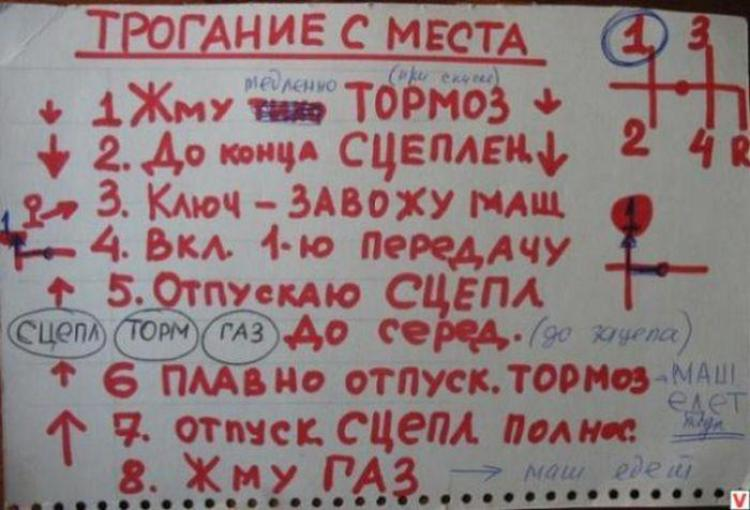
\includegraphics[width=0.9\textwidth]{images/algo_woman_car.jpg}}
\end{frame}

\subsection{Крестики-нолики}
\begin{frame}
  \begin{center}
    \Large{Известно, что в крестики-нолики 3x3 у ноликов есть беспроигрышная стратегия. Опишите её алгоритм.}
  \end{center}
\end{frame}


\subsection{Свойства алгоритма}
\begin{frame}
  \begin{center}
    \Huge{Свойства алгоритмов}
  \end{center}
\end{frame}

\subsection{Понятность}
\begin{frame}
  \begin{center}
    \Huge{Понятность}
  \end{center}
  \begin{center}
    \Large{Если алгоритм непонятен Исполнителю, тот не сможет его выполнить.}
  \end{center}
\end{frame}

\subsection{Однозначность}
\begin{frame}
  \begin{center}
    \Huge{Однозначность}
  \end{center}
  \begin{center}
    \Large{Каждое действие алгоритма должно трактоваться единственным образом.}
  \end{center}
\end{frame}

\subsection{Дискретность}
\begin{frame}
  \begin{center}
    \Huge{Дискретность}
  \end{center}
  \begin{center}
    \Large{Алгоритм должен быть разбит на маленькие последовательные шаги.}
  \end{center}
\end{frame}

\subsection{Универсальность}
\begin{frame}
  \begin{center}
    \Huge{Универсальность}
  \end{center}
  \begin{center}
    \Large{Алгоритм должен уметь работать с разными исходными данными.}
  \end{center}
\end{frame}

\subsection{Результативность}
\begin{frame}
  \begin{center}
    \Huge{Результативность}
  \end{center}
  \begin{center}
    \Large{Таки должен быть результат!}
  \end{center}
\end{frame}

\subsection{Конечность}
\begin{frame}
  \begin{center}
    \Huge{Конечность}
  \end{center}
  \begin{center}
    \Large{Шагов в алгоритме должно быть всё же ограниченное количество.}
  \end{center}
\end{frame}

\subsection{Нарушения}
\begin{frame}[fragile]
  \frametitle{Какие свойства алгоритма нарушаются?}
  \begin{enumerate}
      \item Чтобы найти квадрат числа, нужно его умножить на соответствующее.
      \item Для того, чтобы посчитать длину прямой, надо к ней прикладывать линейку до тех пор, пока прямая не закончится.
      \item Чтобы найти площадь квадрата со стороной 4, надо 4 умножить 4 = 16.
  \end{enumerate}
\end{frame}

\subsection{Почему в России?}
\begin{frame}[fragile]
  \frametitle{Почему в России всё так?}
  \centerline{
\includegraphics[width=0.8\textwidth]{images/russia.png}}
\end{frame}

\subsection{Алгоритмы 1}
\begin{frame}
  \begin{center}
    \Large{Важное свойство алгоритма: алгоритм позволяет большую задачу разбить на несколько простых и небольших шагов}
  \end{center}
\end{frame}

\section{Исполнитель}

\subsection{Исполнитель}
\begin{frame}[fragile]
  \frametitle{Исполнитель}
  \begin{itemize}
    \item \emph{Исполнитель} --- специальная программа, умеющая делать заданный набор действий и принимающая на вход последовательность команд к выполнению.
    \item Представим себе Исполнителя, которого традиционно называют \emph{Черепашка}.
  \end{itemize}
\end{frame}

\subsection{Черепашка}
\begin{frame}[fragile]
  \frametitle{Черепашка}
  \centerline{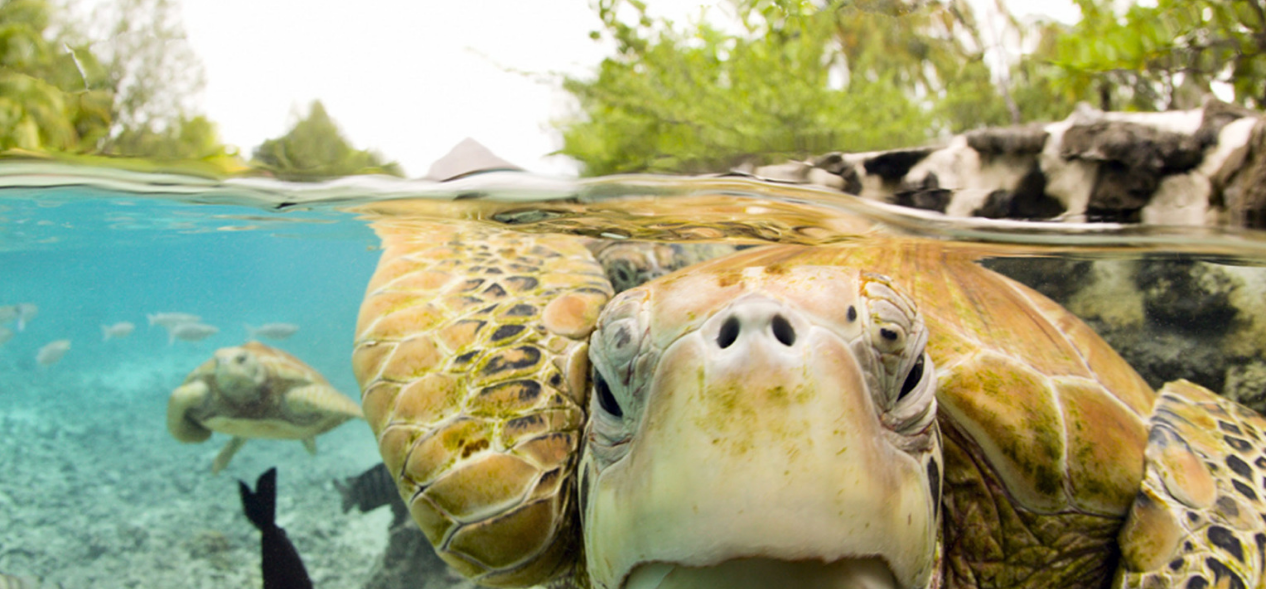
\includegraphics[width=0.9\textwidth]{images/turtle.png}}
\end{frame}

\subsection{Исполнитель Черепашка}
\begin{frame}[fragile]
  \frametitle{Исполнитель Черепашка}
  \begin{itemize}
    \item Черепашка знает следующие команды:
        \begin{enumerate}
            \item ВВЕРХ N --- идти на N шагов вперёд,
            \item ВНИЗ N,
            \item ВПРАВО N,
            \item ВЛЕВО N,
            \item РИСУЙ --- опустить карандаш и рисовать,
            \item НЕ РИСУЙ --- поднять карандаш
        \end{enumerate}
  \end{itemize}
\end{frame}

\subsection{Рисуем квадрат}
\begin{frame}[fragile]
  \frametitle{Рисуем квадрат}
  \begin{itemize}
      \item Напишем алгоритм для рисования квадрата стороной 5:
      \begin{enumerate}
          \item РИСУЙ
          \item ВВЕРХ 5
          \item ВПРАВО 5
          \item ВНИЗ 5
          \item ВЛЕВО 5
      \end{enumerate}
  \end{itemize}
\end{frame}

\subsection{Гоняем черепашку}
\begin{frame}[fragile]
  \frametitle{Гоняем черепашку}
  \begin{itemize}
    \item Напишите алгоритм для рисования:
        \begin{enumerate}
            \item равностороннего треугольника со стороной 5,
            \item буквы С,
            \item буквы Ё,
            \item слова ЙО
        \end{enumerate}
  \end{itemize}
\end{frame}

\subsection{Задача}
\begin{frame}[fragile]
  \frametitle{Задача}
  \begin{itemize}
      \item Исполнитель Черепашка перемещается на экране компьютера, оставляя след в виде линии. В каждый конкретный момент известно положение исполнителя и направление его движения. У исполнителя существуют две команды:
\textbf{Вперёд n}, где n --- целое число, вызывающая передвижение черепашки на n шагов в направлении движения.
\textbf{Направо m}, где m --- целое число, вызывающая изменение направления на m градусов по часовой стрелке.
Запись  \textbf{Повтори 5 [Команда1 Команда2]} означает, что последовательность команд в скобках повторится 5 раз.
Черепашке был дан следующий алгоритм:
\textbf{Повтори 5 [Вперед 10 Направо 72]} Какая фигура появится на экране? 
    \begin{enumerate}
        \item Незамкнутая ломаная линия
        \item Правильный треугольник
        \item Квадрат
        \item Правильный пятиугольник
    \end{enumerate}

  \end{itemize}
\end{frame}

\subsection{Робот}
\begin{frame}[fragile]
  \frametitle{Робот}
  \centerline{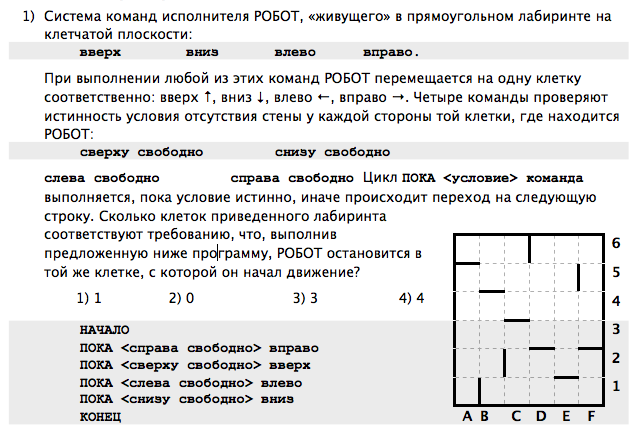
\includegraphics[width=0.8\textwidth]{images/robo.png}}
  
\end{frame}

\end{document}